\chapter{Format of Representative-Number NDI Intervention}
\label{app:format-ndi}

Below is an example format for an NDI-style estimation intervention.  Unlike in
the “evil” NDI intervention, all participants encountered seven or eight such
estimations (described in Appendix~\ref{app:numbers}). Formatting of the survey
items for the web was a straightforward: the statement for each survey item
(provided in Apendix~\ref{app:survey-items}) was provided with a set of radio
buttons directly underneath to allow selection of a response ranging from “1”
(extreme disagreement) to “9” (extreme agreement). Note that I was unable to
capture the actual formatting of the web site used via the Qualtrics system. The
general layout is correct, however the color scheme was UC Berkeley themed. One
detail that is lost occurs where participants are asked to provide percent
confidence: on the web version, there is a slider for that response.

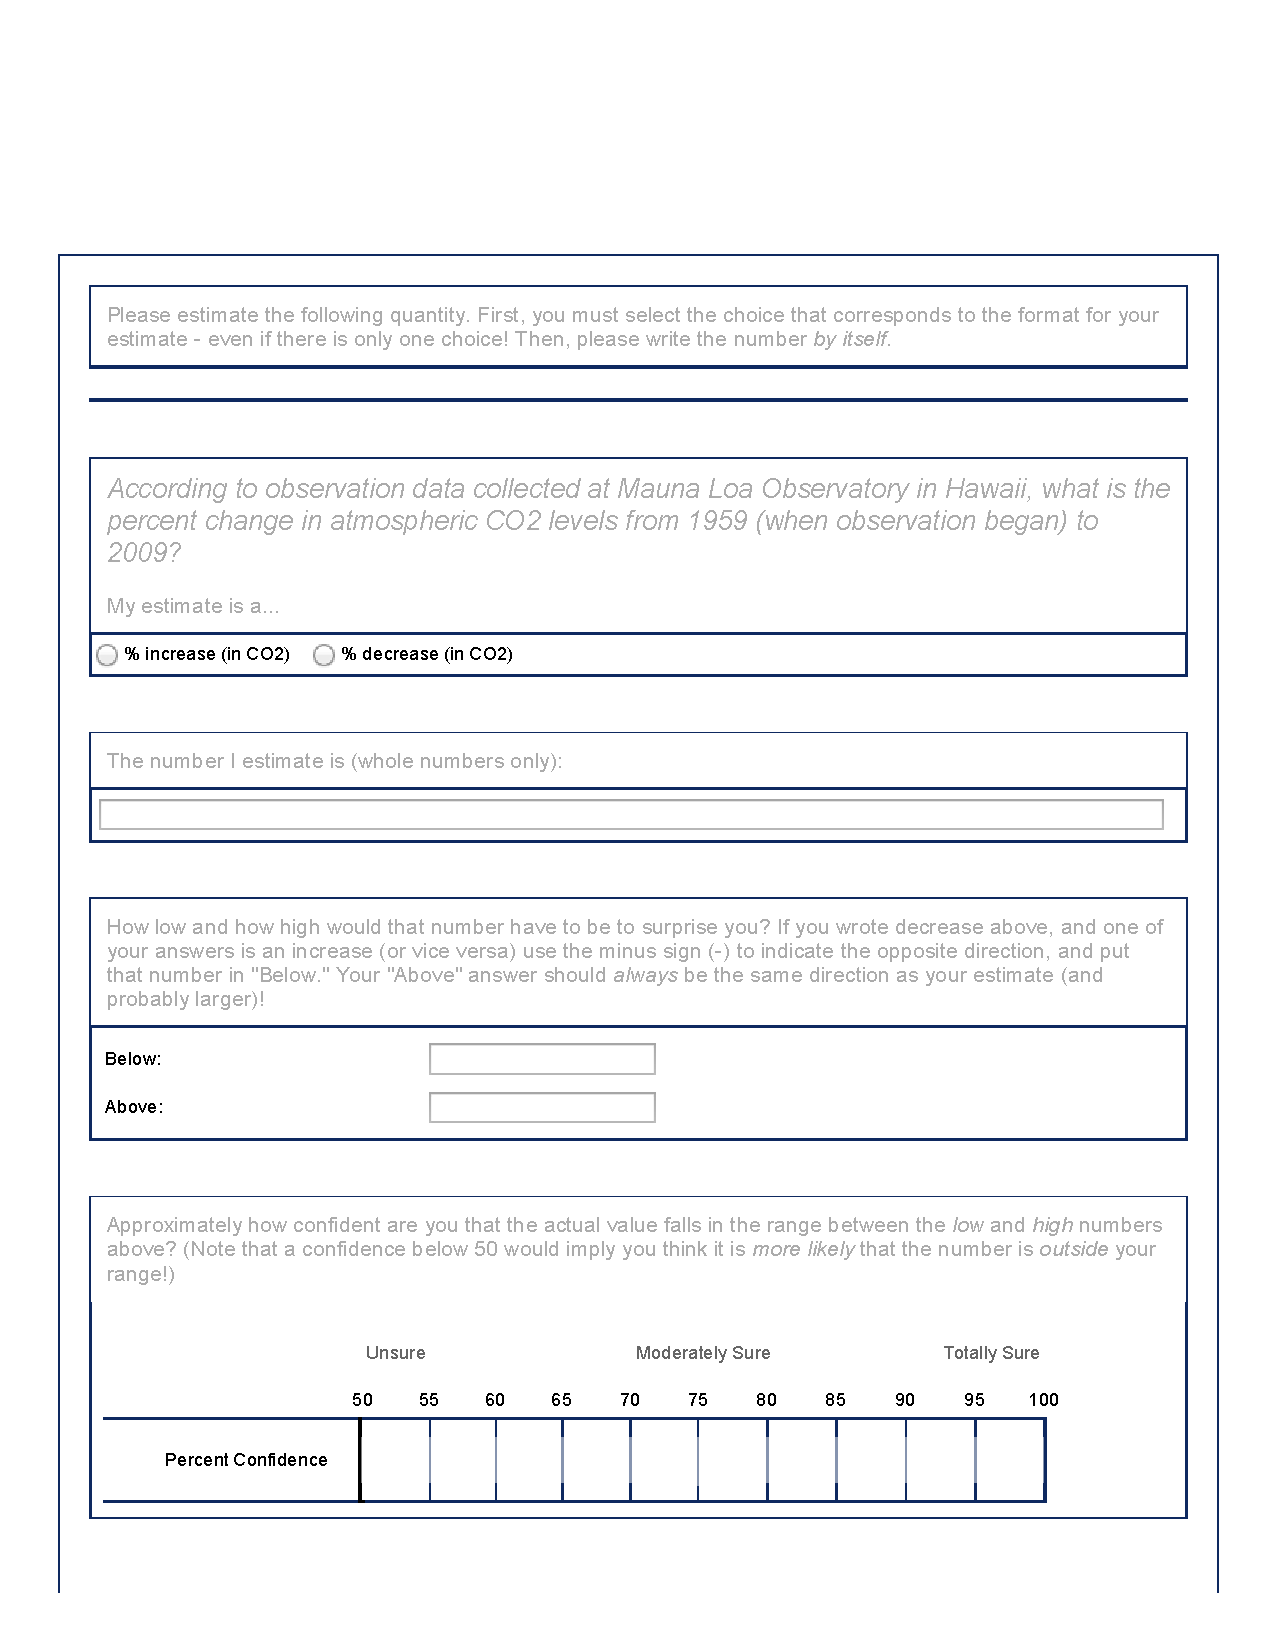
\includepdf[pages=-,pagecommand={},scale=.85]{appendices/Pro-NDI-intervention/Pro-NDI-estimation-example.pdf}
